\documentclass[a4paper,10pt]{ltjsarticle}

% =======================================================================
% パッケージ読込
% =======================================================================

% レイアウト関連パッケージ (geometryなど) は `imp.sty' 内で読込

% 研究発表会・ミーテイング資料用パッケージ
% オプション: 研究発表会用は`presentation',ミーティング用は`meeting'
\usepackage[presentation]{imp}

% 図表関連パッケージ
\usepackage[style=base]{subcaption}
\usepackage{tabularx} % tabularx内でXを指定すると自動で改行してくれる.
\usepackage{graphicx} % 図を描画するために使う.
\usepackage{float} % \begin{figure}[H]でその場に図を出せる

% 数式関連パッケージ
\usepackage{amsmath,amssymb}
\usepackage{bm}
\usepackage{textcomp} % 幾つかの数学記号を使えるようにする
\usepackage{latexsym}

% 箇条書き関連パッケージ
% enumerateやitemizeをもっと使いやすく
% @を箇条書きの深さに
% 最初の50は50個の箇条書きに対応.指定なしだと10以上は使えない.
\usepackage[at,50]{easylist}
\usepackage{enumitem}

% その他のパッケージ
% urlを表示できるようにする
\usepackage{url}
% ハイパーリンクを貼る
\usepackage{hyperref}
% 引用~\citeを拡張.[1,2,3]が[1-3]になる.その他にも機能が.
\usepackage{cite}

% 擬似コード用のパッケージ
\usepackage{algpseudocode, algorithm}

% =======================================================================
% タイトル
% =======================================================================

% 研究発表会の場合
\term{前期}
\date{2022年4月1日}
\group{Learning班}
\grade{B4}
\author{知能メディ夫}
\title{発表タイトル / Presentation Title}

% ミーティングの場合
% 
% \title{Meeting Memo}


% ここまでプリアンブル

% =======================================================================
% 本文
% =======================================================================

\begin{document}
    % タイトルを表示
    \maketitle
    
    % 以下,本文

    \section{使用例}
    \subsection{数式例}
    \verb|\begin{equation}|は使わない.

    数式の改行
    \begin{align}
        a &= \bm{a} + a \nonumber \\
        &=
        \begin{pmatrix}
            1 & 2\\
            3 & 4
        \end{pmatrix}
        \label{eq:equal}
        \\
        a + b + c &= d + e + f
    \end{align}

    こちらは番号がつかない.
    \[
    x=3+4+5
    \]

    数式の参照には\verb|~\eqref|を使う.
    
    式~\eqref{eq:equal}


    \subsection{図の挿入 subcaptionbox}

    \url{http://texdoc.net/texmf-dist/doc/latex/caption/subcaption.pdf}

    captionのwarningの解説.

    \url{ftp://ftp.u-aizu.ac.jp/pub/tex/CTAN/macros/latex/contrib/caption/caption-eng.pdf}

    figureをfigure*にするとtwocolumnでも横いっぱいに広がる.
    tableでも同じ.

    \begin{figure*}[t]
        \centering
        \subcaptionbox{fig3 \label{fig:daisy}}{
            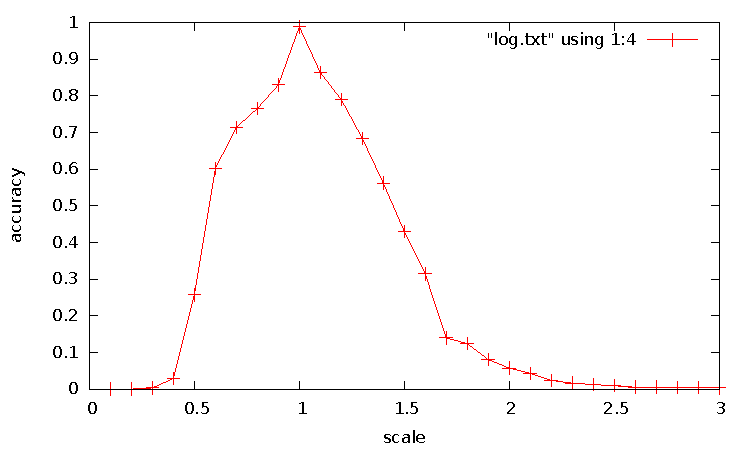
\includegraphics[width=\columnwidth]{./fig/example.pdf}
        }%普通に並べると横に
        \subcaptionbox{fig4 \label{fig:dull}}{
            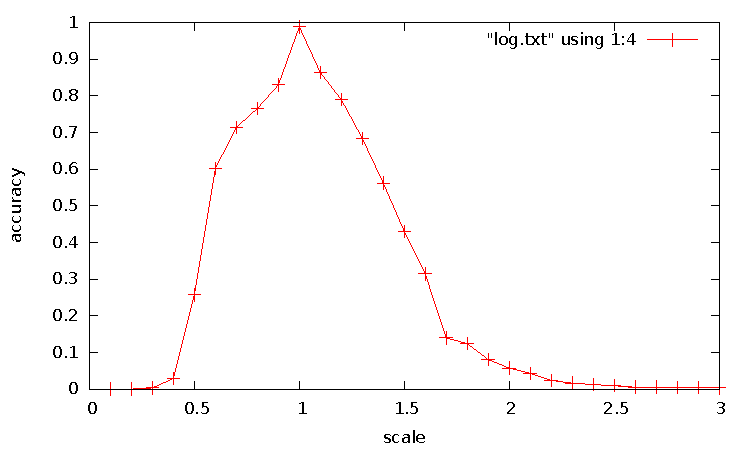
\includegraphics[width=0.5\columnwidth]{./fig/example.pdf}
        }
        \\%改行を入れると下の段に移る
        \subcaptionbox{fig5 \label{fig:aa}}{
            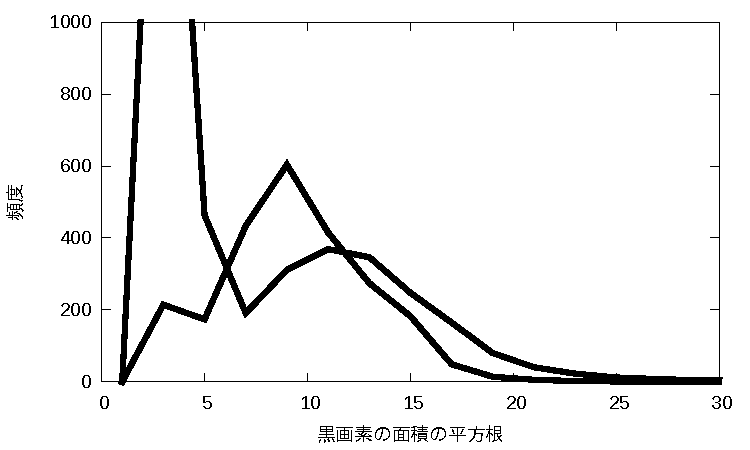
\includegraphics[width=0.5\columnwidth]{./fig/example2.pdf}
        }
        \subcaptionbox{fig6 \label{fig:bb}}{
            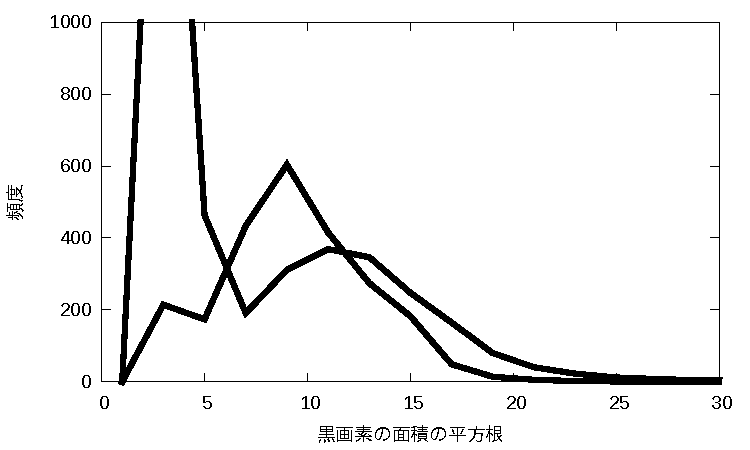
\includegraphics[width=\columnwidth]{./fig/example2.pdf}
        }
        \caption{Wonderful caption Figure~\subref{fig:dull} is fantastic.}
        \label{fig:example}
    \end{figure*}



    \subsection{図の参照}
    キャプションのリファレンスは\verb|~\refと~\subref|で動作が異なる.

    図~\ref{fig:example}

    図~\ref{fig:dull}

    図~\subref{fig:dull}

    \subsection{箇条書き easylist}

    \url{ftp://ftp.u-aizu.ac.jp/pub/tex/CTAN/macros/latex/contrib/easylist/easylist-doc.pdf}


    @の個数によってネストの深さが自動で変わる
    \begin{verb}
    \begin{enumerate}
    \end{verb}
    などのネストをする必要がなくなる.

    easylistのitemizeを利用.
    \begin{easylist}[itemize]
        @ 一段目
        @@ 二段目 \label{nidanme}
        @@@ 三段目
        @@ 二段目に戻った
    \end{easylist}

    itemizeでもラベルと参照は可能.
    ~\ref{nidanme}

    easylistのenumerateを利用.

    \begin{easylist}[enumerate]
        @ 一段目
        @@ 二段目
        @@@ 三段目
        @ 一段目に戻る
    \end{easylist}

    \subsubsection{enumitemの使い方}
    \url{http://konoyonohana.blog.fc2.com/blog-entry-58.html}

    \section{表}
    その結果を表~\ref{tab:foobar}としてまとめる.

    \begin{table*}[t]
        \centering
        \caption{The greatest caption}
        \begin{tabular}{l|rr|rr|rr}
            &\multicolumn{2}{c|}{near} &\multicolumn{2}{c|}{middle} &\multicolumn{2}{c}{ far away}\\
            \hline
            &b&c&d&e&f&g\\
            \hline
            foo &94 &0.41774&97&0.39988&94&0.37474\\
            bar& 84& 0.56925&82&0.66284&78&0.79366 \\
        \end{tabular}
        \label{tab:foobar}
    \end{table*}

    \subsection{疑似コード algpseudocode}
    \begin{algorithm}
        \caption{Compute $aˆb$}
        \begin{algorithmic}[1]
            \State{$c \gets 1$}
            \While{$b \geq 0$}
            \State{$c \gets ac$}
            \State{$b \gets b-1$}
            \EndWhile
        \end{algorithmic}
    \end{algorithm}
    \subsection{その他}

    欄外に脚注

    Google~\footnote{ \url{ http://www.google.co.jp}}

    \subsection{引用}
    文献の参照

    引用例1~\cite{中居2006}.

    複数の引用

    引用例2~\cite{中居2006,ディープラーニング_CVIMチュートリアル,岩村_信学論LLAH2010}.


    \section{参考にしたURL}

    \url{ https://prml.main.ist.hokudai.ac.jp/~ryo/contents/suuri2014/suuri.pdf}

    \url{http://ichiro-maruta.blogspot.jp/2013/03/latex.html}
    
    %\appendix
    %\section{appendixA}
    %これは付録です.

    % 参考文献
    % 参考文献はデフォルトではBibTeXを使用
    \bibliographystyle{junsrt} % 参考文献の表示スタイルを指定.`junsrt', `jplain'などがある.
    {\normalsize % 参考文献のサイズ指定.デフォルトは`\normalsize'.
        \bibliography{index.bib} % 参考文献リスト(.bibファイル)を読み出す.各自で.bibファイルを作成の上読み出すこと.
    }

\end{document}